% $Id: Presentation-CNSTAT2015.tex 1552 2015-05-08 02:38:06Z lv39 $

% normal line:
\documentclass[xcolor=table,compress]{beamer}
% to create notes:
%\documentclass[handout,notes=only]{beamer}
% to create handouts
%\documentclass[xcolor=table,handout,compress]{beamer}
% to create a different kind of handouts
%\documentclass{article}
%\usepackage[envcountsect]{beamerarticle}

%\setbeameroption{handout}
%\setbeameroption{show notes}


%
% Packages
%
\mode<article> % only for the article version
{
  \usepackage{fullpage}
  \usepackage{hyperref}
}
\usepackage{ifpdf}
\ifpdf 
\usepackage{embedfile}
\embedfile{\jobname.tex}
\fi

\usepackage{graphicx}
%\usepackage{pstricks}
\usepackage{pifont}
\usepackage{chicago} 
\newcommand{\citet}{\citeN}
\usepackage{pgf}
\usepackage{amsmath,amssymb,amsfonts}
\usepackage[latin1]{inputenc}
\usepackage{colortbl}
\usepackage[english]{babel}
\usepackage{calc}
%\usepackage{lmodern}
%\usepackage[T1]{fontenc} 

\usepackage{tikz}
\usetikzlibrary{calc}
%\usepackage{qtree}
\usetikzlibrary{shapes,arrows,positioning}

\usepackage{times}
%\usepackage{colortbl}

%============================================================
% Beamer specific styles and configs
%============================================================

\mode<presentation>
{
% alternative, could always use
%\usetheme{Census}
\usetheme{Cornell}
\useoutertheme{Cornell}
}


%\setbeamercovered{dynamic}


%============================================================
% Title
%============================================================

\title[Broadening data access]%
{Broadening data access through synthetic data}
\author[Vilhuber]{%
  Lars~Vilhuber\inst{1} }
\institute[Cornell]{
  \inst{1}%
  
\includegraphics[height=10pt]{cu_logo_only}
    Labor Dynamics Institute, 
   ILR, 
  Cornell University; Cornell NCRN node
%  \and
%  \inst{2}%
%  Center for Economic Studies/LEHD, %\includegraphics[height=7pt]{census-wordmark-transparent}
%  U.S. Census Bureau
}
\date[CNSTAT2015]{NCRN Meetings Spring 2015 @ NAS}
\subject{Synthetic data, LBD, SIPP}

%
% Some useful commands
%

\newcommand{\rarrow}{\selectfont\ding{220}}
\newcommand{\skiplink}{\tiny{\gray\selectfont\ding{59}}}
\newcommand{\goback}{\Acrobatmenu{GoBack}{\gray\selectfont\ding{242}}}
\newcommand{\x}{\selectfont\ding{52}}
\newcommand{\verbatimsize}{\tiny}
\newcommand{\tablesize}{\footnotesize}

\newenvironment{slide}{\begin{frame}}{\end{frame}}
%
% The document proper
%
\begin{document}

\frame{\titlepage
\centering
\tiny with input from John Abowd (NCRN, Cornell), Jerry Reiter (NCRN, Duke), Luke Shaefer (NCRN, Michigan), 
Saki Kinney (NISS), J�rg Drechsler (IAB Germany), Javier Miranda, Martha Stinson, Gary 
Benedetto, Lori Reeder (Census Bureau). Support through NSF Grant SES-0820349, SES-0922005, 
SES-1042181, {\bf SES-1131848}, and Alfred P. Sloan Foundation grant G-2015-13903. 
  }

%\part<presentation>*{Outline}
%
%\begin{frame}
%  \frametitle{Outline}
%  \tableofcontents[part=1,pausesections]
%\end{frame}

% This puts the partial table of contents at the start of each subsection
%\AtBeginSubsection[]
%{
%  \begin{frame}<beamer>
%    \frametitle{Outline}
%    \tableofcontents[current,currentsubsection]
%  \end{frame}
%}


\newcommand{\mytitlepage}[1]{
  \begin{centering}
    {\usebeamerfont{subsection name}\usebeamercolor[fg]{subsection name}}
    \vskip1em\par
    \begin{beamercolorbox}[sep=8pt,center]{part title}
      \usebeamerfont{subsection title}#1
    \end{beamercolorbox}
  \end{centering}
}

\part<presentation>{Main Talk}

%
%  From this point on, we should probably extract it to a sub-document
%

%TCIDATA{Version=5.00.0.2570}
%TCIDATA{LaTeXparent=0,0,Presentation-CAFE-displacement-subdoc.tex}
% $Id: Presentation-CNSTAT2015-subdoc.tex 1552 2015-05-08 02:38:06Z lv39 $
% $URL: https://forge.cornell.edu/svn/repos/ncrn-cornell/branches/papers/CNSTAT2015/text/Presentation-CNSTAT2015-subdoc.tex $

%
%  
%
%\section[Introduction]{Introduction to the paper}

\subsection*{Disclaimer}

\begin{slide}
\frametitle{Disclaimer}
\footnotesize
  \begin{itemize}
  \item Part of the research results were obtained while Vilhuber was a
    Special Sworn Status researcher of the U.S. Census Bureau at the
    Center for Economic Studies.  
    All results have been screened to insure that no confidential data are revealed. 
  \item  Research results and conclusions expressed are those of the authors and
    do not necessarily reflect the views of the Census Bureau. 

  \end{itemize}
\end{slide}


% \begin{frame}
% 	\frametitle{Contents}
% 	\tableofcontents[%
% 		currentsection, % causes all sections but the current to be shown in a semi-transparent way.
% % 		currentsubsection, % causes all subsections but the current subsection in the current section to ...
% % 		hideallsubsections, % causes all subsections to be hidden.
% 		hideothersubsections, % causes the subsections of sections other than the current one to be hidden.
% % 		part=, % part number causes the table of contents of part part number to be shown
% 		pausesections, % causes a \pause command to be issued before each section. This is useful if you
% % 		pausesubsections, %  causes a \pause command to be issued before each subsection.
% % 		sections={ overlay specification },
% 	]
\begin{slide}

  \frametitle{Outline}
  \tableofcontents[part=1,hideallsubsections]
\end{slide}



\section[Background]{Setting the stage}


\newcommand{\mydraws}{  \node[draw, circle, fill=black!10 ] at ({360/\n * (\s - 1)}:\radius) {\label};
  \draw[->, >=latex] ({360/\n * (\s - 1)+\margin}:\radius) 
    arc ({360/\n * (\s - 1)+\margin}:{360/\n * (\s)-\margin}:\radius);
}



\begin{frame}[<+->]{Scope of presentation}
For multitaskers: {\bf goo.gl/zJprV}
\begin{block}{Two synthetic datasets...}
\begin{itemize}[<+->]
\item {\bf Survey of Income and Program Participation (SIPP) Synthetic Beta} (v4 released in 
2009, v5 2010, v6 in March 2015) [SSB]
\item Synthetic Longitudinal Business Database (v2 released 2011) [{\bf SynLBD}]
\end{itemize}
\end{block}
\begin{block}{... or methods ...}
\begin{itemize}[<+->]
\item SynLBD methodology applied to US, German, Canadian data (ongoing)
\end{itemize}
\end{block}
\end{frame}


\begin{frame}[<+->]{Scope of presentation}
\begin{block}{... lessons learned}
\begin{itemize}[<+->]
\item from {\bf Synthetic Data Server} [{\bf SDS}] at {\bf Cornell}  (since 2010)
\end{itemize}
\end{block}
\end{frame}




\begin{frame}
\frametitle{Background}
Creation of analytically valid synthetic data relies on
\begin{block}{Synthetic data feedback loop}
\begin{itemize}[<+->]
\item Create synthetic data
\item Models estimated on synthetic data
\item Models validated on confidential data
\item Lessons learned incorporated into next generation
\end{itemize}
\end{block}
\centering
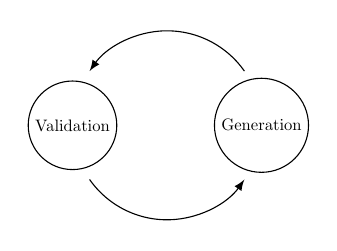
\begin{tikzpicture}[scale=0.6,every node/.style={transform shape}]

\def \n {2}
\def \radius {2cm}
\def \margin {35} % margin in angles, depends on the radius

\def \s {1}
\def \label {Generation}
\onslide<1-4>{  \node[draw, circle ] at ({360/\n * (\s - 1)}:\radius) {\label};}
\onslide<2-4>{  \draw[->, >=latex] ({360/\n * (\s - 1)+\margin}:\radius) 
    arc ({360/\n * (\s - 1)+\margin}:{360/\n * (\s)-\margin}:\radius);}

\def \s {2}
\def \label {Validation}
\onslide<3-4>{  \node[draw, circle ] at ({360/\n * (\s - 1)}:\radius) {\label};
}
\onslide<4>{  \draw[->, >=latex] ({360/\n * (\s - 1)+\margin}:\radius) 
    arc ({360/\n * (\s - 1)+\margin}:{360/\n * (\s)-\margin}:\radius);}

\end{tikzpicture}
\end{frame}




\newcommand{\mydraw}{  \node[draw, circle ] at ({360/\n * (\s - 1)}:\radius) {\label};
  \draw[->, >=latex] ({360/\n * (\s - 1)+\margin}:\radius) 
    arc ({360/\n * (\s - 1)+\margin}:{360/\n * (\s)-\margin}:\radius);
}
\newcommand{\mydrawblue}{  \node[draw, circle, fill=blue!20 ] at ({360/\n * (\s - 1)}:\radius) {\label};}
\newcommand{\mydrawgrey}{  \node[draw, circle, fill=black!10 ] at ({360/\n * (\s - 1)}:\radius) {\label};}
\newcommand{\mydrawline}{  \draw[->, >=latex] ({360/\n * (\s - 1)+\margin}:\radius) 
    arc ({360/\n * (\s - 1)+\margin}:{360/\n * (\s)-\margin}:\radius);
}

\begin{frame}
\frametitle{Background}
\centering
\only<1| handout:0>{
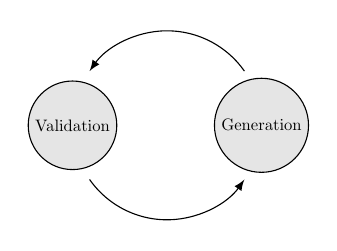
\begin{tikzpicture}[scale=0.6,every node/.style={transform shape}]

\def \n {2}
\def \radius {2cm}
\def \margin {35} % margin in angles, depends on the radius

\def \s {1}
\def \label {Generation}
  \node[draw, circle, fill=black!10 ] at ({360/\n * (\s - 1)}:\radius) {\label};
  \draw[->, >=latex] ({360/\n * (\s - 1)+\margin}:\radius) 
    arc ({360/\n * (\s - 1)+\margin}:{360/\n * (\s)-\margin}:\radius);

\def \s {2}
\def \label {Validation}
  \node[draw, circle, fill=black!10 ] at ({360/\n * (\s - 1)}:\radius) {\label};
  \draw[->, >=latex] ({360/\n * (\s - 1)+\margin}:\radius) 
    arc ({360/\n * (\s - 1)+\margin}:{360/\n * (\s)-\margin}:\radius);



\end{tikzpicture}
}
\only<2-3>{
\begin{tikzpicture}[scale=0.6,every node/.style={transform shape}]

\def \n {6}
\def \radius {3cm}
\def \margin {25} % margin in angles, depends on the radius

\def \s {1}
\def \label {Generation}
\mydrawgrey
\mydrawline

\def \s {2}
\def \label {Learn about}
\only<2>{\mydraw}
\only<3>{\mydrawblue \mydrawline}

\def \s {3}
\def \label {Use SynData}
\only<2>{\mydraw}
\only<3>{\mydrawblue \mydrawline}

\def \s {4}
\def \label {Validation}
\only<2>{\mydrawgrey \mydrawline}
\only<3>{\mydrawblue \mydrawline}

\def \s {5}
\def \label {Extract}
\mydraw

\def \s {6}
\def \label {Learn from}
\mydraw

\end{tikzpicture}
}
\end{frame}



\begin{frame}{Launching synthetic data}
\pause
\includegraphics[width=0.3\textwidth]{baby.jpg}
$\rightarrow$
\onslide<4>{\includegraphics[width=0.3\textwidth]{tricycle2.png}
$\rightarrow$}
\onslide<3->{
\includegraphics[width=0.3\textwidth]{rocket-79468_1280.jpg}}
\end{frame}
\note[enumerate]{\item \url{http://www.peterborough.ca/Assets/City+Assets/Social+Services/Images/Baby+Crawling+to+Laptop.JPG} license unknown
\item \url{http://commons.wikimedia.org/wiki/File:Wisa_Gloria_tricycle_Switzerland_1954.jpg} CC0
\item \url{http://pixabay.com/en/rocket-ship-to-air-blast-off-fire-79468/} CC0
}





\section{Contributions}

\begin{frame}
\frametitle{Contributions}
I will outline the following efforts, including of NCRN nodes:
\tableofcontents[ 
    currentsubsection, 
    hideothersubsections, 
    sectionstyle=show/hide, 
    subsectionstyle=show, 
    ] 
\end{frame}



\subsection[Learning]{Learning about synthetic data}

\begin{frame}
\frametitle{Contributions}
\begin{block}{\begin{tikzpicture}[scale=0.3,every node/.style={transform shape}]
\def \n {6}
\def \radius {3cm}
\def \margin {25} % margin in angles, depends on the radius
\def \s {3}
\def \label {Learn about}
\mydrawblue
\end{tikzpicture}
Focus on learning 
}
In order to get researchers to use the data, they need to know about. 
\end{block}
\pause
\begin{block}{Contributions}
\begin{itemize}[<+->]
	\item Learn about the data

		\begin{itemize}[<+->]
		\item Data documentation 
		\item Provenance
		\end{itemize}
		\onslide<4->{$\rightarrow$ \bf \href{https://www2.ncrn.cornell.edu/ced2ar-web/search}{CED$^2$AR codebooks (Cornell NCRN)}}

	\item Focussed dissemination

		\begin{itemize}[<+->]
		\item Training\onslide<8>{$\rightarrow$ \bf NCRN: Michigan, Duke, Census}
		\item Use in published research\onslide<8>{$\rightarrow$ see \href{http://www2.vrdc.cornell.edu/news/synthetic-data-server/sds-bibliography/}{Cornell website}}
		\item Presentations\onslide<8>{$\rightarrow$ many people}
		\end{itemize}

\end{itemize}
\end{block}

\end{frame}


\begin{frame}
\mytitlepage{Documentation}
\end{frame}


\begin{frame}{Documentation}
\begin{block}{Improving documentation}
\begin{itemize}[<+->]
\item Part of {\bf Cornell NCRN} mission
\item Improve overall availability of documentation
\item Improve controlled availability of documentation on confidential data 
\item Maintain interoperability with other systems (use/expand/influence metadata standards)
\end{itemize}
\end{block}
\end{frame}

%\begin{frame}
%\centering
%\includegraphics[height=0.9\textheight]{Selection_079.png}
%\note{Software to work with standards-enhanced metadata}
%\end{frame}

\begin{frame}
\centering
\includegraphics[height=0.9\textheight]{Selection_080.png}
\note{SSB v6 codebook was entirely developed on CED2AR with NCRN help}
\end{frame}

\begin{frame}
\centering
\includegraphics[height=0.9\textheight]{Selection_082.png}
\note{SynLBD is derived from LBD}
\end{frame}



\begin{frame}<handout:0>{Goal}
\centering
\includegraphics[height=0.8\textheight]{LBD_Provenance.png}
\end{frame}

\begin{frame}{Goal}
\begin{columns}[T]
\begin{column}{0.45\textwidth}
\begin{itemize}[<+->]
\item {\bf Derive} the provenance graph from existing information
\item {\bf Simplify} the procedures
\item Work within {\bf existing} standards
\end{itemize}
\end{column}
\begin{column}{0.55\textwidth}
\includegraphics[width=\textwidth]{LBD_Provenance.png}

\end{column}

\end{columns}
\end{frame}



\begin{frame}
\mytitlepage{Teaching}
\end{frame}

\begin{frame}{Teaching}
\begin{block}{Advanced Workshop on SIPP Synthetic Beta}
\href{http://www.ncrn.info/event/advanced-workshop-sipp-synthetic-beta-ssb}{\includegraphics[height=0.6\textheight]{Selection_083.png}}
\end{block}
\end{frame}

\begin{frame}{Teaching}
\begin{block}{PAA Workshop on SIPP}
\href{http://www.ncrn.info/event/workshop-redesign-survey-income-and-program-participation}{\includegraphics[height=0.6\textheight]{Selection_088.png}}
\end{block}
\end{frame}

\begin{frame}{Teaching}
\begin{block}{Workshops on SIPP Synthetic Beta}
\begin{itemize}
\item Part of the activities of {\bf Michigan and Triangle NCRN node}
\item Additional support from {\bf Cornell}
\item Integrated into workshops, summer schools, conferences (12 participants, June 2014; 
several dozen at  PAA, April, 2015)
\end{itemize}
\end{block}
\end{frame}


\begin{frame}{Teaching}

\mytitlepage{Synthetic data is really useful for graduate research}

\end{frame}



\begin{frame}{Teaching}

\begin{block}{Use of synthetic data for graduate research}
\begin{itemize}
\item Wait times for thesis projects using confidential data may be long (months to years)
\item Wait times for SDS accounts substantially shorter (1-2 weeks)
\item Statistical agency has fast turnaround on validation (often 1-2 weeks, depending on 
complexity)
\item Anecdotal evidence of substantial use of SDS projects by students
\item Two theses using the synthetic data, several others in progress
\end{itemize}
\end{block}
\end{frame}





\begin{frame}
\mytitlepage{Graduate students are the ambassadors}
\end{frame}






























\subsection[Use]{Encouraging use of synthetic data}

\begin{frame}
\mytitlepage{\insertsubsection}
\end{frame}


\begin{frame}
\frametitle{Contributions}
\begin{block}{\begin{tikzpicture}[scale=0.3,every node/.style={transform shape}]
\def \n {6}
\def \radius {3cm}
\def \margin {25} % margin in angles, depends on the radius
\def \s {3}
\def \label {Use}
\mydrawblue
\end{tikzpicture}
Focus on use}
In order to get researchers to use the data, it needs to be convenient and useful.
\end{block}
\pause
\begin{block}{Contributions}
\begin{itemize}[<+->]
	\item Allow researchers to work as close as possible to their regular workflow

		\begin{itemize}[<+->]
		\item Ideally, downloadable data (desktop paradigm)
		\item If not, server-based desktop paradigm with easy access 
		\end{itemize}
		\onslide<4->{$\rightarrow$ \textbf{Synthetic Data Server (Cornell)}}

\end{itemize}
\end{block}

\end{frame}


%\begin{frame}{What does that mean?}
%\begin{block}{Using the Synthetic Data Server}
%\centering
%
%\includegraphics[height=0.8\textheight]{screenshot-SDSx.png}
%\end{block}
%\end{frame}


\begin{frame}{How has that worked?}
\begin{block}{Usage of Synthetic Data Server}
\centering

\includegraphics[height=0.8\textheight]{report_on_SDS_2015-accounts.pdf}
\end{block}
\end{frame}


\begin{frame}{Remember...}
\includegraphics[width=0.3\textwidth]{baby.jpg}
\end{frame}




\begin{frame}{How has that worked?}
\begin{block}{User profile and Census RDC contact}
\centering
\only<1| handout:0>{
\includegraphics[height=0.75\textheight]{report_on_SDS_2015-useRDCgraph-edited.png}}
\only<2>{\includegraphics[height=0.75\textheight]{report_on_SDS_2015-useRDCgraph.pdf}}

\note{Thanks to Barbara Downs, Census Bureau}
\end{block}
\end{frame}




\begin{frame}{How has that worked?}
\begin{block}{Additional pathways}
\begin{itemize}[<+->]
\item Not only a valid data analytic tool ...
\item ... additional pathway to confidential data \note{while waiting for access to RDC}
\item ... with better utility than other ``test'' data \note{Such as in Germany or Canada}
\end{itemize}
\end{block}
\end{frame}







\subsection[Validation]{Facilitating validation}
\begin{frame}
\mytitlepage{\insertsubsection}
\end{frame}

\begin{frame}
\frametitle{Contributions}
\begin{block}{\begin{tikzpicture}[scale=0.3,every node/.style={transform shape}]
\def \n {6}
\def \radius {3cm}
\def \margin {25} % margin in angles, depends on the radius
\def \s {3}
\def \label {Validation}
\mydrawblue
\end{tikzpicture}
Focus on validation methods}

\end{block}

\begin{block}{Validation for statistical agencies}
\begin{itemize}
	\item Validation is a cost, to be balanced against alternate access mechanisms
	\item Cheaper is better

\end{itemize}
\end{block}
\begin{block}{Validation for researchers}
\begin{itemize}
	\item Validation is a cost, to be balanced against alternate access mechanisms
	\item Faster is better
\end{itemize}
\end{block}

\end{frame}


\begin{frame}{Statistics}
\begin{block}{Hard metrics are hard to come by}
In December 2012,  out of {\bf 30 users} of the {\bf SynLBD}, 3 users had generated {\bf 5 
validation} requests.
\end{block}
\begin{block}{Other outcomes}
\begin{itemize}
\item Some users have ``self-validated'' by going into the RDC
\item Some users have ``kicked the tires'' 
\end{itemize}
\end{block}
\pause
\onslide<2>\includegraphics[width=0.3\textwidth]{baby.jpg}

\end{frame}


%\begin{frame}{An example: Bertrand, Kamenica, Pan (2015)}
%\begin{block}{Study on relative income within households}
%\centering
%\includegraphics[height=0.9\textheight]{Bertrand-QJE-2015-FigureIII.png}
%\end{block}
%\end{frame}
%
%
%\begin{frame}{An example: Bertrand, Kamenica, Pan (2015)}
%\begin{block}{Project with SIPP Synthetic Beta}
%\centering
%\includegraphics[height=0.8\textheight]{jma_graph_rel_earn3_syn.png}
%\end{block}
%\end{frame}
%
%\begin{frame}{An example: Bertrand, Kamenica, Pan (2015)}
%\begin{block}{Validation against Gold Standard SIPP file}
%\centering
%\includegraphics[height=0.8\textheight]{jma_graph_rel_earn3.png}
%\end{block}
%\end{frame}


\begin{frame}[<+->]{Making validation easier}
\begin{block}{Key insight}
\centering
validation = replication
\end{block}

\begin{block}{Solution}
\centering
Use workflow tools
\end{block}

\begin{block}{Key problem}
\centering
social scientists don't like workflow tools
\end{block}

\end{frame}

% % % % % % % % % 
%

\begin{frame}{Our solution}
\begin{block}{Ex-post workflow documentation}
\begin{itemize}[<+->]
\item Within a restricted-access environment (RDC) or a validation-requirement environment (SDS), user is required to document end results
\item Already includes (i) description of variables (ii) description of programs used to generate variables (iii) description of transformations
\item {\bf Cornell NCRN}: same data documentation standard as used for codebook generation
\item ... with one twist: addition of PROV language

\end{itemize}
\end{block}
\end{frame}


\tikzstyle{entity} = [rectangle, rounded corners , minimum height=4em, draw, fill=yellow!20, 
    text width=4.5em, text badly centered,  inner sep=0pt]
\tikzstyle{block} = [rectangle, draw, fill=blue!20, 
    text width=5em, text centered, rounded corners, minimum height=4em]
\tikzstyle{line} = [draw, -latex']
\tikzstyle{cloud} = [draw, ellipse,fill=red!20,
    minimum height=2em]


\begin{frame}{DDI+PROV for workflow}
\begin{tikzpicture}[auto,
	scale=0.6,every node/.style={transform shape},
	myscope/.style={node distance=1em and 0em}]
    % Place nodes
    \node [cloud] (dataw) {Data Warehouse};
    \node [entity, right=5em of dataw] (LBD) {LBD};
    \node [block, fill=black!20, right=4em of LBD] (program) {Program};
    \node [entity, below=4em of program] (results) {Results};
    \node [right=8em of results] (placeh) {};
\only<2->{    \node [star, star points=7, draw, fill=blue!20, below=8em of dataw](DDI) {DDI};}
\only<3->{    \node [star, star points=7, draw, fill=blue!20, above=12em of placeh](PROV) {PROV};}
    % Draw edges
\only<1-2>{
    \path [line]  (dataw) -- node  {hadMember} (LBD) ;
    \path [line] (program) -- node  {used} (LBD) ;
    \path [line] (results) -- node  {isGeneratedby} (program);}
\only<2->{    \path [line,color=blue] (DDI) -- (LBD);
    \path [line,color=blue] (DDI) -- (results);}
\only<3>{
    \path [line]  (dataw) -- node [text=red] (l1) {hadMember} (LBD) ;
    \path [line] (program) -- node [text=red]  (l2) {used} (LBD) ;
    \path [line] (results) -- node [text=red]  (l3) {isGeneratedby} (program);
    \path [line, color=red] (PROV) -- (l1);
    \path [line, color=red] (PROV) -- (l2);
    \path [line, color=red] (PROV) -- (l3);
    }

\end{tikzpicture}

\end{frame}    


\begin{frame}{How to create this?}
\begin{block}{You've seen something like this before:}

\includegraphics[height=0.9\textheight]{Selection_082.png}
\end{block}

\end{frame}


\begin{frame}{How to create this?}


\includegraphics[height=0.9\textheight]{Selection_086.png}

\end{frame}



\begin{frame}{Example release request}
\begin{columns}[T]
\begin{column}{0.49\textwidth}
\includegraphics[width=\textwidth]{RDCDisclosureRequestMemo.pdf}
\end{column}\pause
\begin{column}{0.49\textwidth}
\includegraphics[width=\textwidth]{SYNLBDV2_Disclosure_CED2AR.pdf}
\end{column}
\end{columns}
\end{frame}

\begin{frame}{Why does this matter?}
\begin{block}{Machine-actionable documents}
From the same document...
\begin{itemize}[<+->]
\item ... generate result release request  \textit{(which the user needed to generate anyway)}
\item ... generate programs for validation \textit{ (which the statistical agency needs anyway)}
\item ... database the analyses for later meta-analysis \textit{(helping in the extraction of models 
and 
results)}
\end{itemize}
\end{block}
\end{frame}

\subsection{International expansion}

%\begin{frame}
%\frametitle{Contributions}
%\begin{block}{\begin{tikzpicture}[scale=0.3,every node/.style={transform shape}]
%\def \n {6}
%\def \radius {3cm}
%\def \margin {25} % margin in angles, depends on the radius
%\def \s {3}
%\def \label {Use}
%\mydrawblue
%\end{tikzpicture}
%Focus on use}
%In order to get researchers to use the data, it needs to be convenient and useful.
%\end{block}
%\pause
%\begin{block}{Contributions}
%\begin{itemize}[<+->]
%	\item Expand applications and data coverage is one way of enhancing utility to researchers, 
%	and possibly statistical agencies
%
%		\begin{itemize}[<+->]
%		\item \textit{German Synthetic LBD}	(Work by Drechsler and Vilhuber)
%		\item[{$\rightarrow$}] \textbf{Cornell}, IAB Germany
%	    \item \textit{Canada} (tentative, grant proposal)
%		\item[{$\rightarrow$}] \textbf{Cornell, Duke}, others
%		\item other countries (some expression of interest)
%		\end{itemize}
%
%\end{itemize}
%\end{block}
%
%\end{frame}

\note[enumerate]{

	\item[{$\rightarrow$}] contributes to "Learning from"
	\item[{$\rightarrow$}] greater utility for researchers on SDS (cross-country analysis)
	\item[{$\rightarrow$}] greater utility for researchers: existence of cross-national comparable confidential data files (cross-country analysis)
}



\begin{frame}
\frametitle{Contributions}
\begin{block}{\begin{tikzpicture}[scale=0.3,every node/.style={transform shape}]
\def \n {6}
\def \radius {3cm}
\def \margin {25} % margin in angles, depends on the radius
\def \s {3}
\def \label {Use}
\mydrawblue
\end{tikzpicture}
Focus on use}
In order to get researchers to use the data, it needs to be convenient and useful.
\end{block}
\pause
\begin{block}{Contributions}
\begin{itemize}[<+->]
	\item Expanding to international context


	\item[{$\rightarrow$}] contributes to \begin{tikzpicture}[scale=0.3,every 
	node/.style={transform shape}]
	\def \n {6}
	\def \radius {3cm}
	\def \margin {25} % margin in angles, depends on the radius
	\def \s {3}
	\def \label {Learning from}
	\mydrawblue
	\end{tikzpicture} (robustness of synthetic data models)
	\item[{$\rightarrow$}] greater utility for researchers: existence of cross-national comparable 
	confidential data files (cross-country analysis)
\end{itemize}
\end{block}

\end{frame}

%
% ============= Conclusion =================
%
%
\section{Conclusion}
\label{sec:Conclusion}

\begin{frame}
\frametitle{Conclusion}
\begin{block}{Still early}
\begin{itemize}
\item Still countable users
\item Expansion will require some automation, ranging from making complex manual processes 
easier, to full automation (Duke)
\item Acceptance is a big part of the equation: more examples are needed, greater scope of 
application, more training
\item Cost effectiveness still hard to assess, but critical for agency buy-in
\end{itemize}
\end{block}
\end{frame}

\begin{frame}
\frametitle{}
\begin{block}{Thank you.}

\end{block}
\end{frame}
\ifpdf
\embedfile{\jobname-subdoc.tex}
\fi

%\part<presentation>{Appendix}

%%TCIDATA{Version=5.00.0.2570}
%TCIDATA{LaTeXparent=0,0,Presentation-CAFE-displacement-subdoc.tex}
% $Id: Presentation-CNSTAT2015-appendix.tex 1541 2015-05-03 01:57:12Z lv39 $
% $URL: https://forge.cornell.edu/svn/repos/ncrn-cornell/branches/papers/CNSTAT2015/text/Presentation-CNSTAT2015-appendix.tex $

% Stuff here that need not go in the main presentation
% such as bibliography, additional tables
 

\begin{slide}
\frametitle{References}
\tiny
\bibliographystyle{chicagoa} 
\bibliography{abbrev,\jobname.bib}
\end{slide}
\ifpdf
\IfFileExists{\jobname.bib}{\embedfile{\jobname.bib}}{}
\IfFileExists{abbrev.bib}{\embedfile{abbrev.bib}}{}
\fi




%
% Reference to itself
%

\begin{frame}[fragile]
{\huge The end}
\vfill
\verbatimsize
\begin{verbatim}
 $Id: Presentation-CNSTAT2015-appendix.tex 1541 2015-05-03 01:57:12Z lv39 $
\end{verbatim}
\end{frame}




%\ifpdf
%\embedfile{\jobname-appendix.tex}
%\fi

\end{document}


